% Chapter 1
%\newcommand {\DF}[2]{{\displaystyle\frac{#1}{#2}}}
\chapter{Tunnelling Spectroscopy with Proximity Effect} % Write in your own chapter title
\label{Chapter3}
\lhead{Chapter 3. \emph{Tunnelling Spectroscopy with Proximity Effect}} % Write in your own chapter title to set the page header

It is interesting to propose a theory calculating the $d$-wave conductance accounting for the proximity effect as required by our novel experiments.

Identical to the steps mentioned in the last chapter. We first solve the Bogoliubov equations and study the properties of the the tunnelling conductance kernel, $\sigma_S$ in (2.25). Then the knowledge of the conductance kernel, $\sigma_S$ will guide us to the desired $d$-wave proximity conductance.
Currently this work is in progress.
\section{Bogoliubov Equations}
As a matter of fact, the tunnelling conductance discussed in the previous chapter is based on a specific case which is shown in Fig.2.2. The potential is assumed as a $\delta$ function and the pair potential is assumed as a step function, so that Bogoliubov  equations(3.1) have an analytical solution. In contrast, such analytical solution no longer exists when dealing with more complicated case accounting for proximity effect.
\subsection{Simplification for Bogoliubov Equations}
The general Bogoliubov equations are 
\begin{eqnarray}
i\hbar\frac{\partial f}{\partial t} = \Big(-\frac{\hbar^2}{2m}\frac{\partial^2}{\partial {x^2}}-\mu(x)+V(x)\Big)f(x,t)+\Delta(x)g(x,t)\nonumber\\
\\
i\hbar\frac{\partial g}{\partial t} = \Big(-\frac{\hbar^2}{2m}\frac{\partial^2}{\partial {x^2}}-\mu(x)+V(x)\Big)g(x,t)+\Delta(x)f(x,t)\nonumber
\end{eqnarray}
(3.1) has the solution form 
\begin{eqnarray}
\varphi(x,t)=
\left(\begin{array}{c}
f(x,t)\\
g(x,t)
\end{array}\right)
\end{eqnarray}
where $\mu(x),\Delta(x),V(x)$ are chemical potential, energy gap, and the ordinary potential which is related to barrier hight, in which we are interested in the latter two.
By introducing a solution of the form
\begin{eqnarray}
f=u(x)e^{ik_Fx-\frac{iEt}{\hbar}}\nonumber\\
\\
g=v(x)e^{ik_Fx-\frac{iEt}{\hbar}}\nonumber\
\end{eqnarray}
The Bogoliubov equations could be written in this way neglecting higher order terms\citep{Reference4}.
\begin{eqnarray}
&&\DF{\partial u}{\partial x}=i(\pi \xi_0\Delta_{\infty})^{-1}[Eu-\Delta(x)v]\nonumber\\
&&\\
&&\DF{\partial v}{\partial x}=-i(\pi \xi_0\Delta_{\infty})^{-1}[Ev-\Delta(x)u]\nonumber
\end{eqnarray}
which are the equations we are interested in, $\xi_0$ is the coherence length. Also we have the accompanied boundary conditions
\begin{eqnarray}
&&\varphi^+=\varphi^-\nonumber\\
\\
&&\frac{\partial \varphi^+}{\partial x}-\frac{\partial \varphi^-}{\partial x}=2k_FZ\varphi^+\nonumber
\end{eqnarray}

The tunnelling axis is divided into four regions\citep{Reference4}, named 'super','reduced','induced','normal', respectively, which is shown in Fig.3.1, where we already choose parabolic shape for the pair potential.
As indicated in the reference\citep{Reference4}, the Bogliubov equations are solved region by region, which finally lead us to the tunnelling conductance kernel. The andreev reflection $A$ and ordinary reflection $B$ in (3.6) could be directly calculated from the solutions from the Bogliubov equations.
\begin{eqnarray}
\sigma_S=1+A-B
\end{eqnarray}

\section{Analysis of the Solutions of Bogoliubov Equations}
\subsection{The Shapes of Reduced and Induced Pair Potential}
To be precise we need to compute the pair potential using self-consistent method\citep{Reference11}. Yet we won't lose two much information if we only guess the shape of the pair potential\citep{Reference8, Reference4}. We are using parabolic shape of pair potential which is like Fig.3.1

Another point we should account for is the proximity thickness, which will affect much the shape of the computed results. We define
\begin{eqnarray}
x_S=a_S\pi\xi_0,x_N=a_N\pi\xi_0\nonumber\\
\\
\xi_0=\hbar^2 k_F/(\pi\Delta_{\infty})\nonumber
\end{eqnarray}
where in effect we find only the factors $a_S,a_N$ play the role of influencing the results.
Therefore, we choose the potential function as 
\begin{eqnarray}
&&\Delta_R(x)=\frac{\Delta_r-\Delta_{\infty}}{x_S^2}(x-x_S)^2+\Delta_{\infty}\nonumber\\
&&\\
&&\Delta_I(x)=\frac{\Delta_i}{x_N^2}(x+x_S)^2\nonumber
\end{eqnarray}
who have the shapes in Fig.3.1.
Now let us first study some intermediate values in the calculation.
\subsection{Shapes of $|u|,|v|$}
We  take a look at the shapes of $|u|,|v|$, which are also affected by the chosen energy value $E$ and if not noted, the bulk potential is always set to $\Delta_{\infty}=1$
\begin{figure}[htbp]
\small
	\centering
		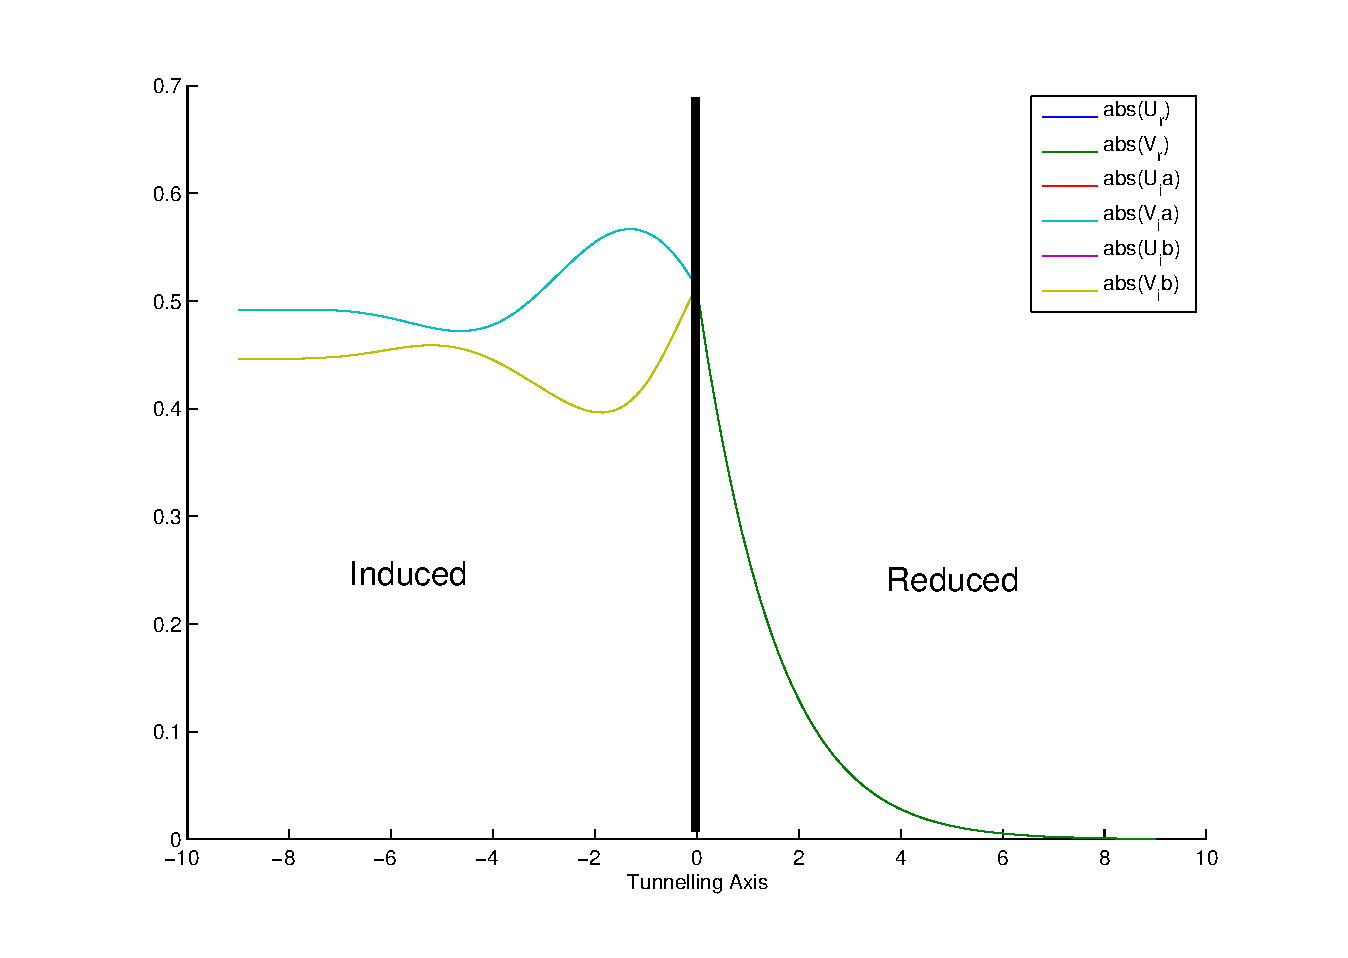
\includegraphics[width=10cm]{./Figures/3-2-2.eps}
		\rule{35em}{0.5pt}
	\caption[An Electron]{The shapes with $E=0.5$, subscript $r$ indicates reduced region while $i$ induced region. Notice that in reduced region, $u^*=v$.}
	\label{fig:Electron}
\end{figure}
 \begin{figure}[htbp]
\small
	\centering
		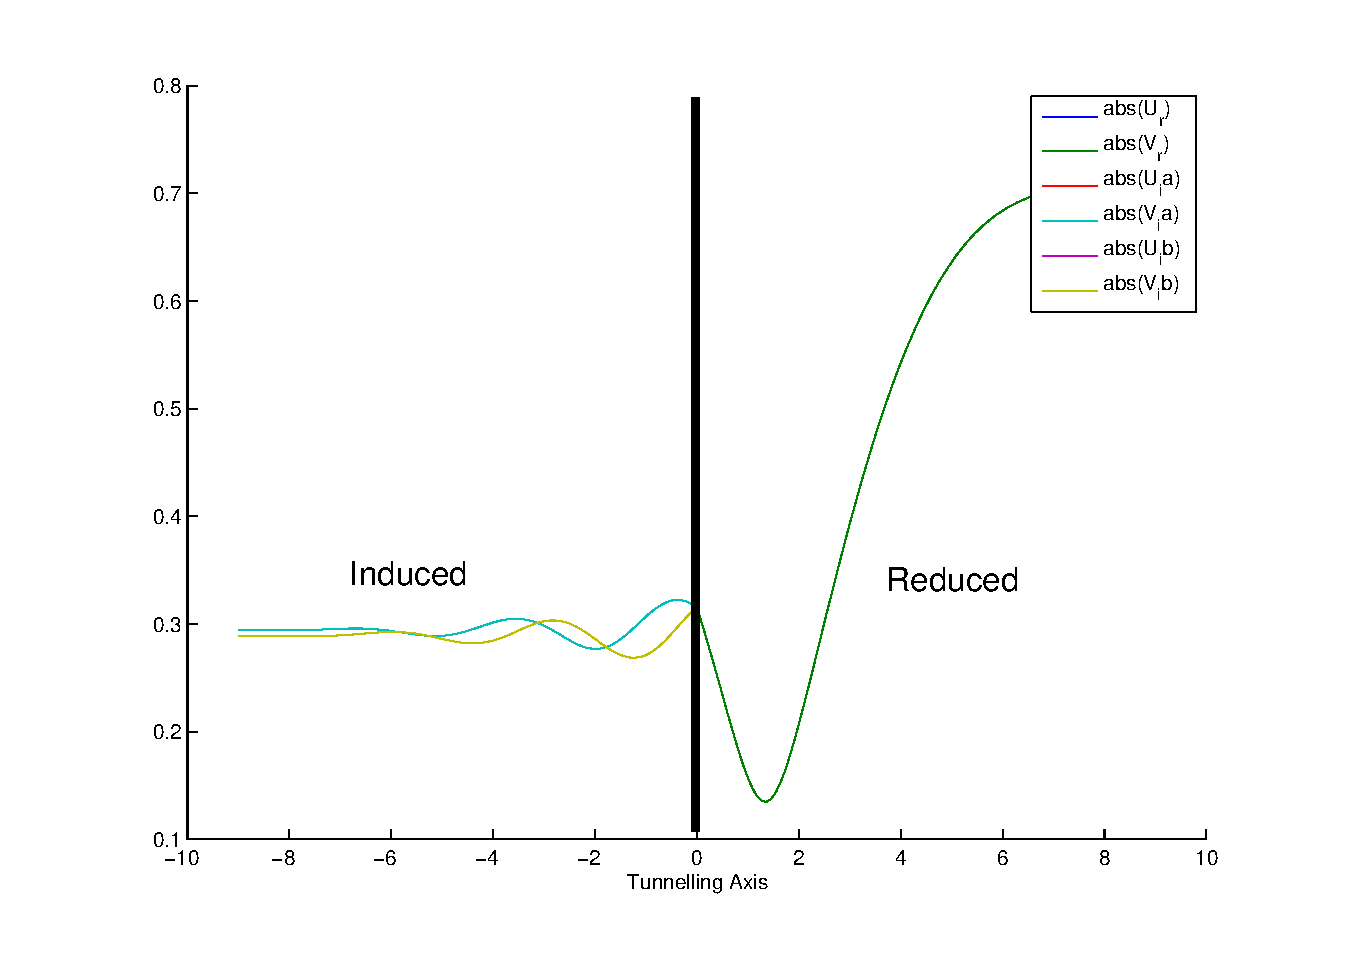
\includegraphics[width=10cm]{./Figures/3-2-3.eps}
		\rule{35em}{0.5pt}
	\caption[An Electron]{The shapes with $E=1$, subscript $r$ indicates reduced region while $i$ induced region}
	\label{fig:Electron}
\end{figure}

 \begin{figure}[htbp]
\small
	\centering
		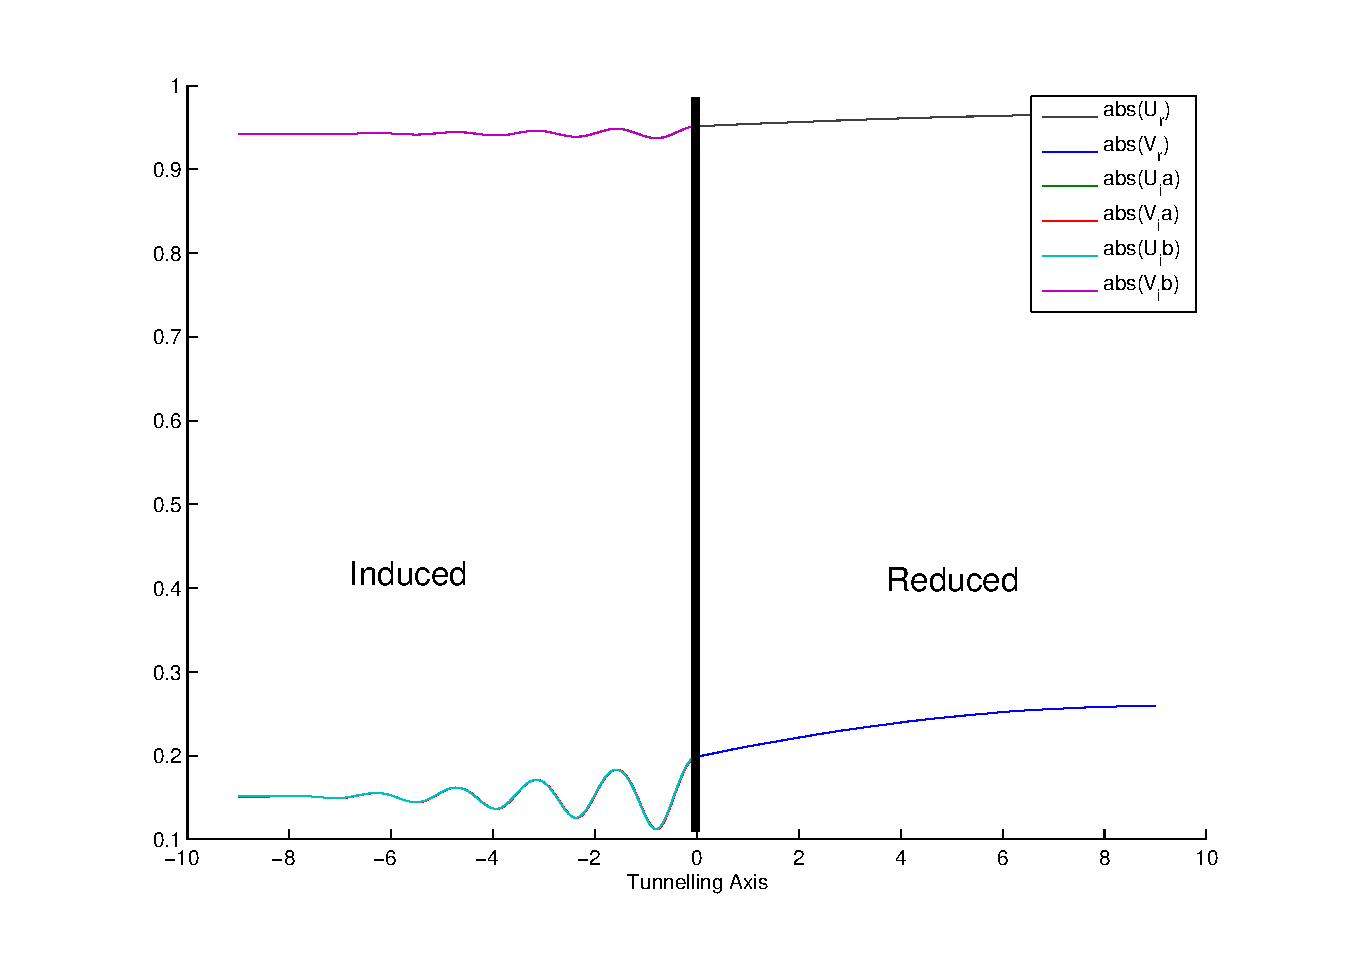
\includegraphics[width=10cm]{./Figures/3-2-4.eps}
		\rule{35em}{0.5pt}
	\caption[An Electron]{The shapes with $E=2$, subscript $r$ indicates reduced region while $i$ induced region}
	\label{fig:Electron}
\end{figure}

 \subsection{The Specific Case of BTK}
 First of all we check the reliability of our model. Ideally, BTK is a specific case of our discussion in this chapter; in other words, if we set $\Delta_R=1,\Delta_I=0$, we should see the results of BTK, Fig3.5.
Here are a set of figures, in which the deep blue one represents the BTK, the famous V-shape shown.
\begin{figure}[htbp]
\small
	\centering
		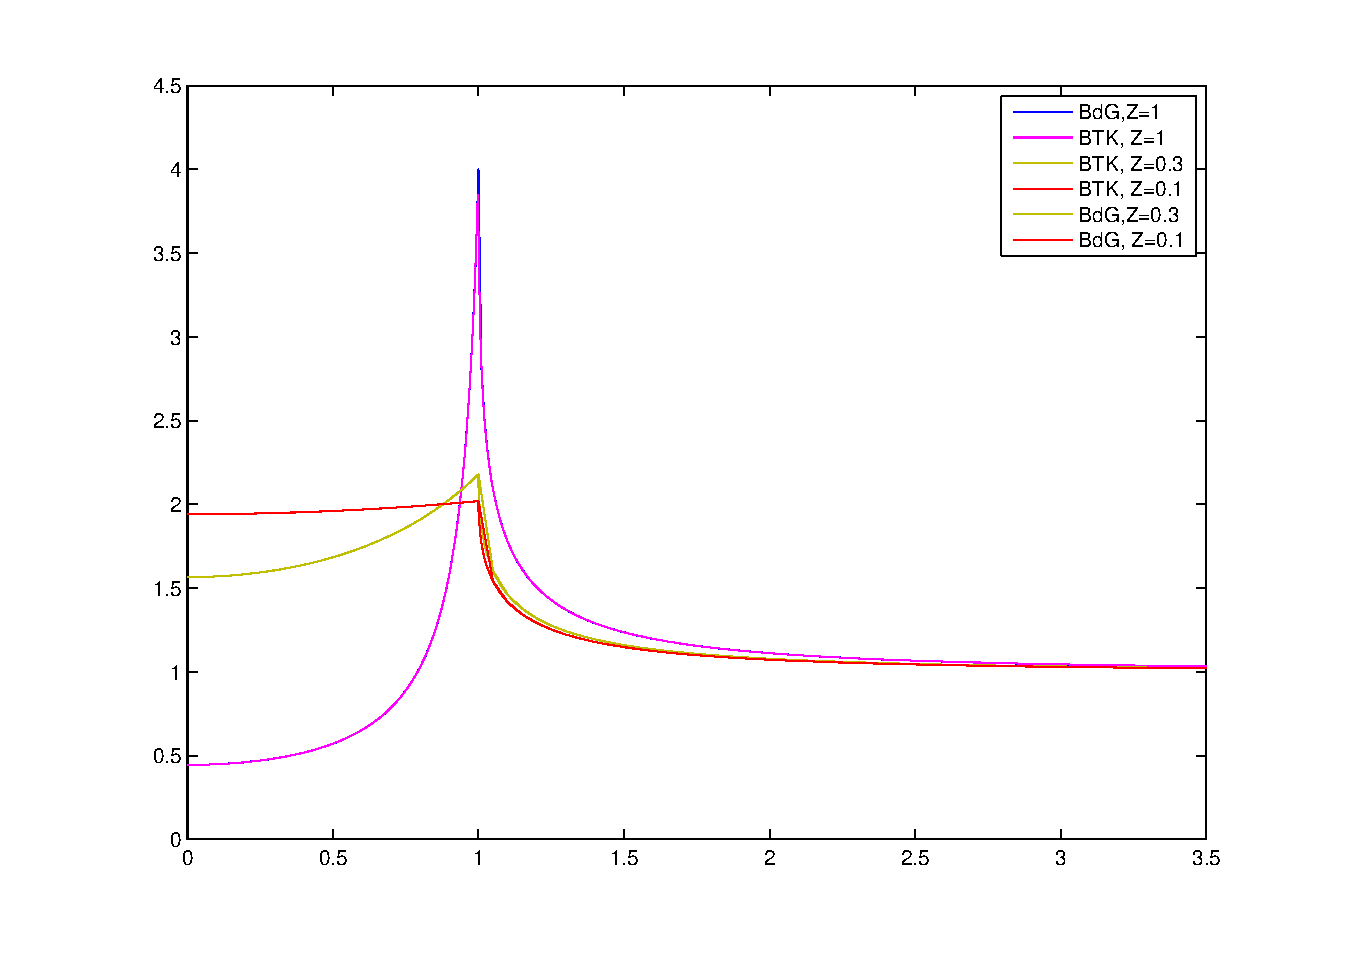
\includegraphics[width=10cm]{./Figures/3-2-8.eps}
		\rule{35em}{0.5pt}
	\caption[An Electron]{BTK case when we set $\Delta_R=1,\Delta_I=0$}
	\label{fig:Electron}
\end{figure}
 Also, when barrier hight $Z=0$, we should observe flat region with the value of $2$ in the middle, Fig.3.6.
\begin{figure}[htbp]
\small
	\centering
		\includegraphics[width=10cm]{./Figures/3-2-9.eps}
		\rule{35em}{0.5pt}
	\caption[An Electron]{The flat region in the middle appears no matter what parameters we set}
	\label{fig:Electron}
\end{figure}

\section{Tunnelling Spectroscopy with Proximity Effect}
Similar to the procedure in the previous chapter, with solutions obtained, we first have a look at the kernel of the conductance.
\begin{eqnarray}
\sigma_T=1+A-B
\end{eqnarray}

\subsection{$s$-wave Tunnelling Spectroscopy with Proximity Effect}
From the Bogoliubov equations we get the tunnelling conductance kernel, $\sigma_S$, which determines the properties of the tunnelling spectroscopy (3.10).
\begin{eqnarray}
\sigma_T(E)=\DF{\int_0^{2\pi}d\varphi\int_{-\frac{\pi}{2}}^{\frac{\pi}{2}}d\theta \sigma_S(E)\cos\theta}{\int_{0}^{2\pi}d\varphi\int_{-\frac{\pi}{2}}^{\frac{\pi}{2}}d\theta\sigma_N\cos\theta}
\end{eqnarray}

If we set the $\Delta_{\infty}$ independent of angle, the results obtained from (3.10) represent $s$-wave tunnelling spectroscopy.

In Fig.3.6, we set bulk gap $\Delta_{\infty}=2$, fix the reduced gap$\Delta_r=1$ and vary the induced gap $\Delta_i$ from $0$ to $1.5$.  The red tongue in the middle indicates the properties of the varying induced gap, whose width is from $0$ to about $1.5$, corresponding to the value of induced gap at that point.
\begin{figure}[htbp]
\small
	\centering
		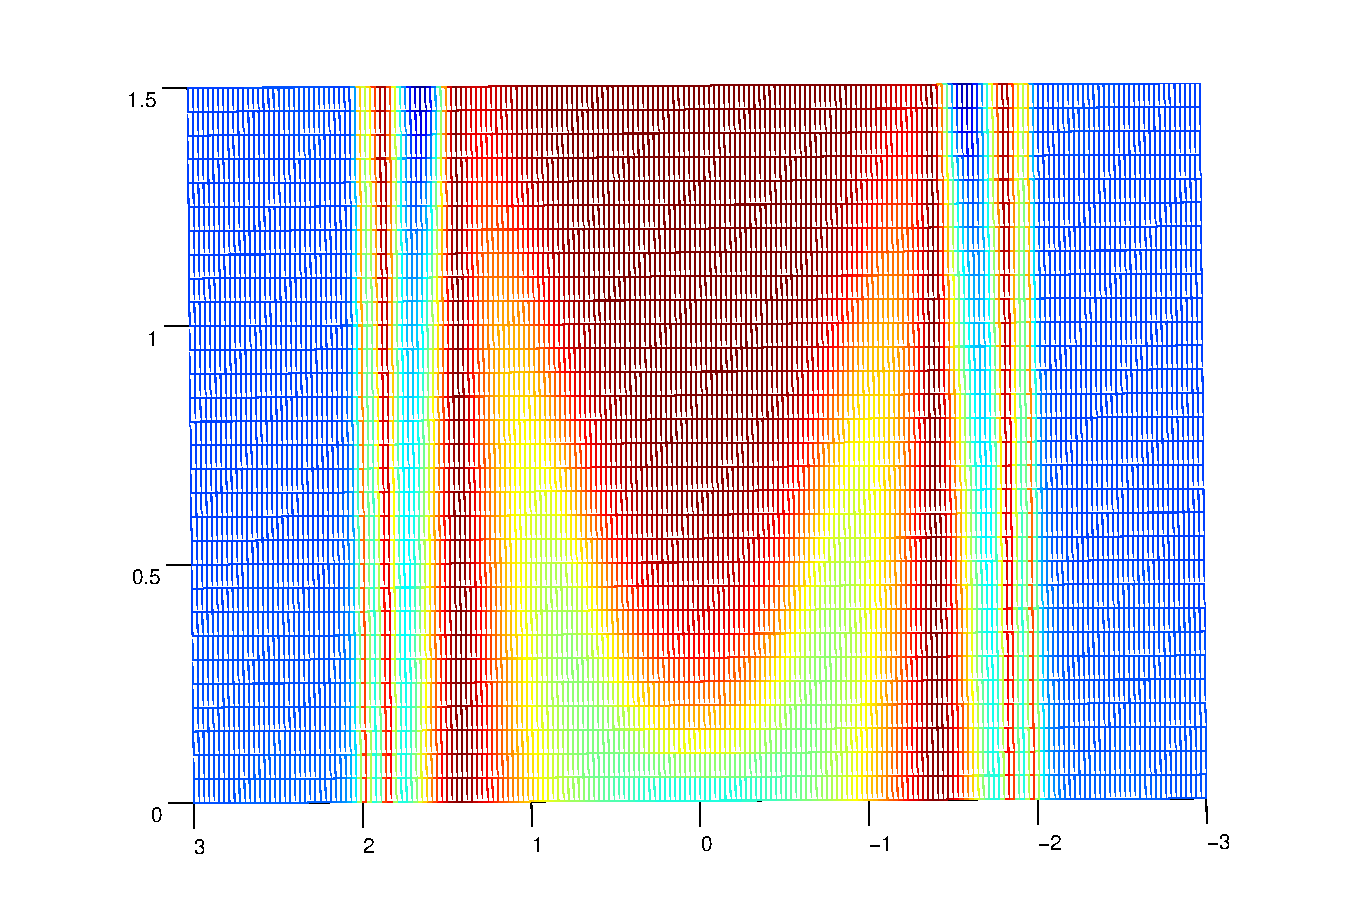
\includegraphics[width=10cm]{./Figures/3dinduce.eps}
		\rule{35em}{0.5pt}
	\caption[An Electron]{The picture shows the properties of the tunnelling conductance when induced gap is varying while reduced gap is fixed. The blue colour indicates the low conductance value while in contrast the red colour indicates the high conductance value.}
	\label{fig:Electron}
\end{figure}

In Fig.3.7, we set bulk gap $\Delta_{\infty}=2$, fix the reduced gap$\Delta_i=0.4$ and vary the induced gap $\Delta_r$ from $0$ to $2$.  The red rectangular with $width=0.8$ shows the existence of the induced gap. The two branches growing from the bottom indicates the existence of the reduced gap. The minimum value of the reduced gap in the bottom seems to be expelled by the induced gap that it could not reach $0$ as it should be. The maximum value of the reduced gap is at $1$ as it should be.
\begin{figure}[htbp]
\small
	\centering
		\includegraphics[width=12cm]{./Figures/3dreduceinduce.pdf}
		\rule{35em}{0.5pt}
	\caption[An Electron]{The picture shows the properties of the tunnelling conductance when the reduced gap is varying while the induced gap is fixed. The blue colour indicates the low conductance value while in contrast the red colour indicates the high conductance value.}
	\label{fig:Electron}
\end{figure}

\subsection{A Brief Introduction to $d$-wave Tunnelling Spectroscopy with Proximity Effect}
Our work at $d$-wave tunnelling spectroscopy with proximity effect is currently in progress. When moving into $d$-wave case, first of all the $\Delta_{\infty}$ in (3.4) is no longer independent of angle, but has to follow the assumption (2.5). In $d_{x^2-y^2}$ $c$-tunnelling case, we assume that the terms in (3.8)
\begin{eqnarray}
\Delta_{\infty}=\Delta_{\infty0}\cos(2\varphi)\nonumber\\
\Delta_r=\Delta_{r0}\cos(2\varphi)\\
\Delta_i=\Delta_{i0}\cos(2\varphi)\nonumber
\end{eqnarray}
Another change resulted from the assumption (3.11) is that the factors $a_S, a_N$ in term (3.7) are now related to the angle.
\begin{eqnarray}
a_S=\frac{x_S}{\pi\xi_0}=\frac{x_S\Delta_{\infty}}{\hbar^2k_F}\sim\cos(2\varphi)\nonumber\\
\\
a_N=\frac{x_N}{\pi\xi_0}=\frac{x_N\Delta_{\infty}}{\hbar^2k_F}\sim\cos(2\varphi)\nonumber\
\end{eqnarray}
Different from the discussion in the previous chapter, the $d$-wave tunnelling spectroscopy is quite distinct from the $c$-tunnelling spectroscopy when proximity effect is introduced. A surface reason is that the factors $a_S, a_N$ affect the shape of the tunnelling spectroscopy heavily.










